\documentclass{article}
\usepackage{tikz}
\usetikzlibrary{angles,quotes,patterns,arrows.meta,positioning,calc}

\begin{document}

\title{TikZ Feladatok}
\author{Vadon Viktória \\ 2023/24/I. félév}
\date{}
\maketitle

\section*{1. Feladat – Házikó}

\subsection*{a) alapok}
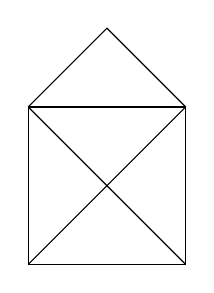
\begin{tikzpicture}
    \draw (0,0) -- (2,0) -- (2,2) -- (0,2) -- cycle;
    \draw (0,0) -- (2,2);
    \draw (0,2) -- (2,0);
    \draw (0,2) -- (1,3) -- (2,2);
\end{tikzpicture}

\subsection*{b) egy vonallal
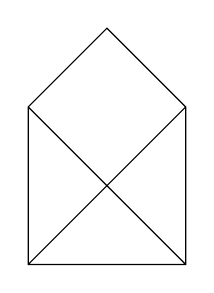
\begin{tikzpicture}
    \draw (0,0) -- (2,0) -- (2,2) -- (1,3) -- (0,2) -- cycle
          (0,0) -- (2,2) (0,2) -- (2,0);
\end{tikzpicture}

\subsection*{c) nagyitva}

\begin{tikzpicture}[scale=2]
    \draw (0,0) -- (2,0) -- (2,2) -- (1,3) -- (0,2) -- cycle
          (0,0) -- (2,2) (0,2) -- (2,0);
\end{tikzpicture}

\section*{2. Feladat}

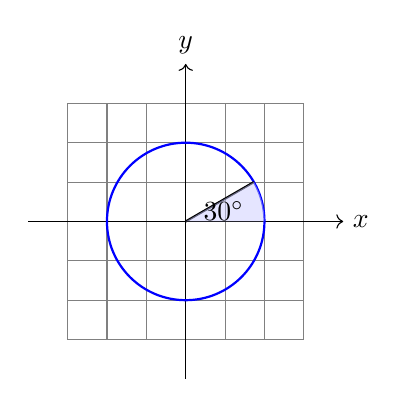
\begin{tikzpicture}
    \draw[step=0.5,gray,thin] (-1.5,-1.5) grid (1.5,1.5);
    \draw[->] (-2,0) -- (2,0) node[right] {$x$};
    \draw[->] (0,-2) -- (0,2) node[above] {$y$};
    \draw[thick,blue] (0,0) circle (1);
    \draw[thick] (0,0) -- (cos 30, sin 30);
    \begin{scope}
        \fill[blue!20, opacity=0.5] (0,0) -- (1,0) arc (0:30:1) -- cycle;
    \end{scope}
    \draw (15:0.5) node {$30^\circ$};
\end{tikzpicture}

\section*{3. Feladat}

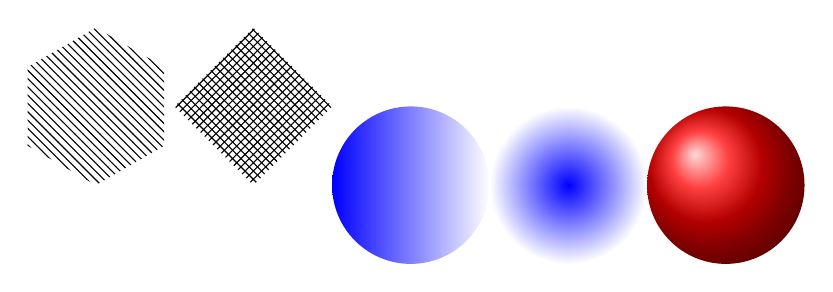
\begin{tikzpicture}
    \fill[pattern=north west lines] (0,0) -- ++(30:1) -- ++(90:1) -- ++(150:1) -- ++(210:1) -- ++(270:1) -- ++(330:1) -- cycle;
    \begin{scope}[xshift=2cm]
        \fill[pattern=crosshatch] (0,0) -- ++(1,1) -- ++(-1,1) -- ++(-1,-1) -- cycle;
    \end{scope}
    \begin{scope}[xshift=4cm]
        \shade[left color=blue, right color=white] (0,0) circle (1);
    \end{scope}
    \begin{scope}[xshift=6cm]
        \shade[inner color=blue, outer color=white] (0,0) circle (1);
    \end{scope}
    \begin{scope}[xshift=8cm]
        \shade[ball color=red] (0,0) circle (1);
    \end{scope}
\end{tikzpicture}

\newpage

\section*{4. Feladat}

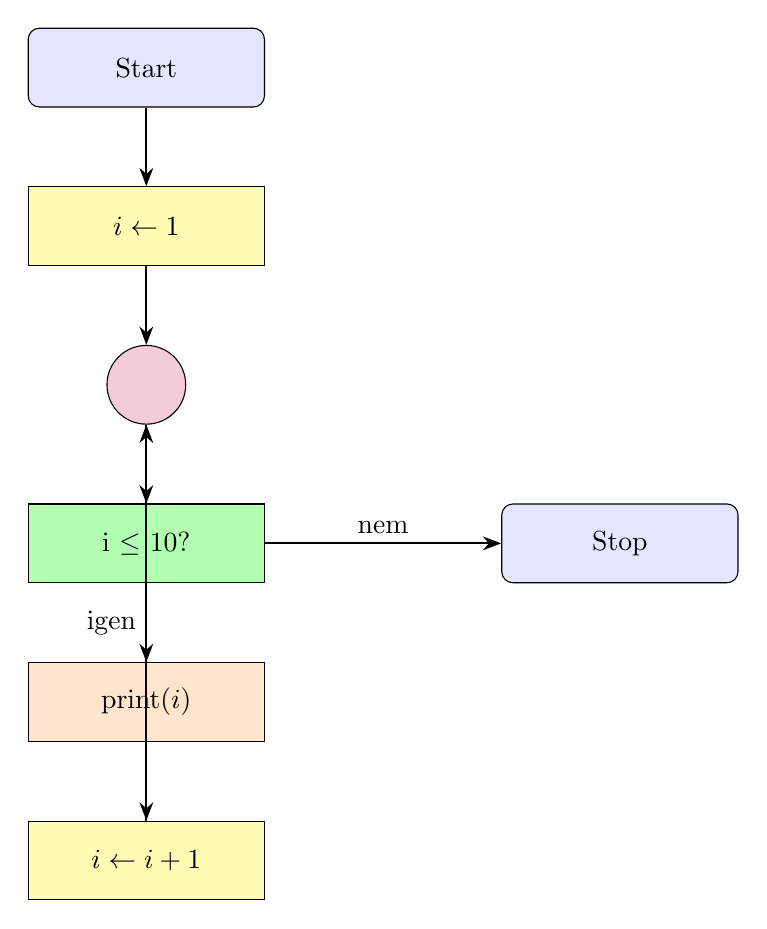
\begin{tikzpicture}[
    startstop/.style={rectangle, rounded corners, draw, fill=blue!10, minimum width=3cm, minimum height=1cm},
    process/.style={rectangle, draw, fill=yellow!30, minimum width=3cm, minimum height=1cm},
    decision/.style={rectangle, draw, fill=green!30, minimum width=3cm, minimum height=1cm, inner sep=0pt, align=center},
    io/.style={rectangle, draw, fill=orange!20, minimum width=3cm, minimum height=1cm, align=center},
    arrow/.style={-Stealth, thick}
]

\node (start) [startstop] {Start};
\node (init) [process, below=of start] {$i \leftarrow 1$};
\node (loop) [circle, draw, fill=purple!20, minimum size=1cm, below=of init] {};
\node (check) [decision, below=of loop] {i $\leq$ 10?};
\node (print) [io, below=of check] {print($i$)};
\node (inc) [process, below=of print] {$i \leftarrow i + 1$};
\node (stop) [startstop, right=3cm of check] {Stop};

\draw [arrow] (start) -- (init);
\draw [arrow] (init) -- (loop);
\draw [arrow] (loop) -- (check);
\draw [arrow] (check) -- node[anchor=east] {igen} (print);
\draw [arrow] (print) -- (inc);
\draw [arrow] (inc) -- ++(0,1.5) -| (loop);
\draw [arrow] (check) -- node[anchor=south] {nem} (stop);
\end{tikzpicture}

\newpage

\section*{5. Feladat}

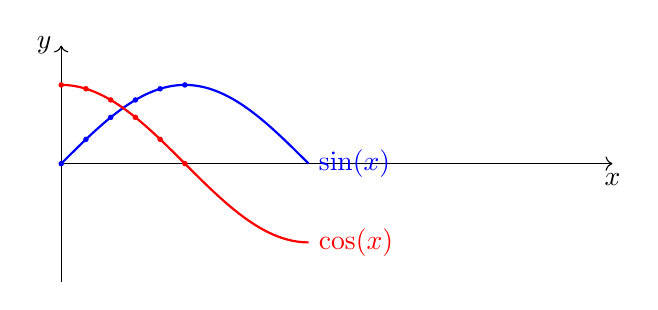
\begin{tikzpicture}
    \draw[->] (0,0) -- (7,0) node[below] {$x$};
    \draw[->] (0,-1.5) -- (0,1.5) node[left] {$y$};

    \draw[blue, thick, domain=0:3.14159] plot[samples=100] (\x, {sin(\x r)}) node[right] {$\sin(x)$};
    \draw[red, thick, domain=0:3.14159] plot[samples=100] (\x, {cos(\x r)}) node[right] {$\cos(x)$};

    \foreach \x in {0, 0.314, 0.628, 0.942, 1.256, 1.57} {
        \fill[blue] (\x, {sin(\x r)}) circle (1pt);
    }
    \foreach \x in {0, 0.314, 0.628, 0.942, 1.256, 1.57} {
        \fill[red] (\x, {cos(\x r)}) circle (1pt);
    }
\end{tikzpicture}

\newpage

\section*{6. Feladat}

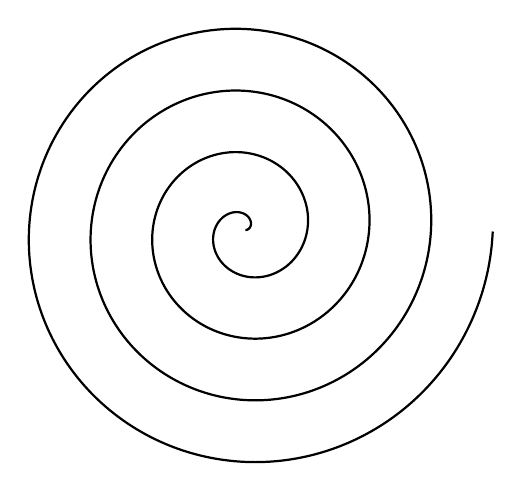
\begin{tikzpicture}
    \draw[domain=0:8*pi, variable=\t, smooth, samples=500, thick] 
        plot ({\t/8 * cos(\t r)}, {\t/8 * sin(\t r)});
\end{tikzpicture}

\end{document}

